% AR-Politeia Cycle 1 -- PRL-format condensed journal draft
% Written by the journal_prl isolated writing agent from:
%   research/orchestration/comprehensive.json
%   research/findings.json
%   rules/journal-formats.md
% Status: negative / inconclusive cycle; no confirmatory scientific claim is made.

\documentclass[aps,prl,reprint,superscriptaddress,amsmath,amssymb]{revtex4-2}

\usepackage[T1]{fontenc}
\usepackage[utf8]{inputenc}
\usepackage{graphicx}
\usepackage{tikz}
\usetikzlibrary{arrows.meta,positioning,calc,fit,backgrounds,decorations.pathreplacing}
\usepackage{booktabs}
\usepackage{xcolor}
\usepackage{microtype}

\definecolor{accent}{RGB}{20,72,130}
\definecolor{warn}{RGB}{160,40,40}
\definecolor{ok}{RGB}{20,120,70}
\definecolor{grey}{RGB}{90,90,90}

\begin{document}

\title{Numerical calibration halts a preregistered matched-landscape test of resource autocorrelation in a minimal Langevin socioeconomic model}

\author{AR-Politeia Collaboration}
\affiliation{AutoResearcher Project \texttt{ar-politeia}, Cycle 1}
\date{\today}

\begin{abstract}
We report a preregistered numerical study of whether the spatial arrangement of a resource landscape---rather than its total, marginal distribution, or accessible area---changes steady-state population aggregation and wealth structure in a minimal fixed-population Langevin agent model. The confirmatory stage was not reached. The calibration gate completed 25 runs and passed wealth conservation (maximum relative drift $2.51\times10^{-9}$), non-negativity, and equal-state absorption, but failed time-step convergence and stationarity; the wealth Gini coefficient changed by $0.26584885869833064$ between $\mathrm{d}t/2$ and $\mathrm{d}t/4$, above the preregistered limit of $0.02$. Consequently claim C1-NUM is contradicted, claims C2--C4 are inconclusive, and the landscape, channel-ablation, and robustness experiments were blocked before execution. We preserve this negative result and recommend an outcome-blind parameter-lock revision and recalibration before any confirmatory claim.
\end{abstract}

\maketitle

\section{Introduction}

A central question in the statistical mechanics of socioeconomic organization is whether the spatial arrangement of resources matters once the total endowment and its marginal distribution are fixed \cite{duran2025, bae2026}. Pattern-oriented agent modeling suggests that such questions should be tested against multiple predeclared observables, and uncertainty quantification argues for separating numerical validity from substantive inference \cite{grimm2005, mcculloch2022}. Here we take that distinction literally. We implement a minimal Langevin agent model in which the landscape can affect agents through two switchable channels---movement and local wealth production---and ask whether clustered versus exactly shuffled resource fields produce a measurable population-structure difference.

Our principal result is negative at the numerical level, not at the scientific level. The preregistered calibration gate failed on time-step convergence and stationarity, so the confirmatory landscape contrast was correctly blocked before execution. We therefore cannot yet answer the core question; we also must not report the blocked experiments as a null landscape effect. The value of the letter is the explicit demonstration that a generative model can be designed with machine-checked causal matching and hard gate stops, and that the stop itself identifies an actionable failure mode: the wealth dynamics are not yet discretization-converged in the tested window.

\section{Minimal model and physical picture}

Each agent has a position $(x_i,y_i)$, momentum $(p_{x,i},p_{y,i})$, and wealth $w_i$; the ability $\epsilon_i$ is frozen to one and population is fixed, so demography and ability evolution cannot act as hidden confounders. Positions and momenta follow a Br\"unger--Brooks--Karplus (BBK) Langevin update,
\begin{equation}
\mathrm{d}p = F\,\mathrm{d}t-\gamma p\,\mathrm{d}t+\sqrt{2\gamma m k_B T}\,\mathrm{d}W,
\qquad
\frac{\mathrm{d}x}{\mathrm{d}t}=\frac{p}{m},
\label{eq:langevin}
\end{equation}
where $F$ is the deterministic terrain force, $\gamma$ is friction, and $T$ is temperature. The noise amplitude is fixed by the fluctuation--dissipation relation, but no social fluctuation--dissipation law is asserted. Equation \eqref{eq:langevin} has a simple physical reading: agents are pulled toward resource gradients, slowed by friction, and kicked by thermal noise. With $\gamma=1$, $T=0.5$, $k_B=1$, and $m=1$, motion is inertial but overdamped; when both friction and noise are switched off the integrator reduces to deterministic Velocity--Verlet.

Wealth is transferred in pairwise encounters with a label-symmetric, saturating rule,
\begin{equation}
A_i=\epsilon_i\frac{w_i}{w_i+w_{\mathrm{ref}}},
\qquad
\Delta w=\eta\,\frac{A_i-A_j}{A_i+A_j}\min(w_i,w_j),
\label{eq:exchange}
\end{equation}
where the transfer is from $j$ to $i$. The pair update is antisymmetric under exchange, so aggregate wealth is conserved and inequality arises from state differences rather than from a biased rule. The half-saturation scale $w_{\mathrm{ref}}=5$ keeps the transfer bounded at large wealth. Local production changes wealth through
\begin{equation}
\mathrm{d}w_i=R(x_i)\epsilon_i\,\mathrm{d}t-c\,\mathrm{d}t-d\,w_i\,\mathrm{d}t,
\qquad
R(x)=\mathrm{base\_production}\cdot\mathrm{scale}\cdot\max(0,-V(x)).
\label{eq:production}
\end{equation}
In the intended confirmatory regime $\mathrm{base\_production}=0.01$, while consumption $c$ and decay $d$ are zero. The two terrain channels are therefore independently switchable: \texttt{terrain\_force\_enabled} controls whether the resource gradient moves agents, and \texttt{terrain\_production\_enabled} controls whether resource depth produces wealth. Culture, technology, reproduction, mortality, loyalty, conquest, taxation, and polity classification are disabled in Cycle 1.

\section{Preregistered design and claims}

The causal design fixes total resources, pixel-value histogram, accessible area, population, and initial wealth while varying only spatial autocorrelation. A clustered field is generated as five anisotropic Gaussian bumps with lognormal amplitudes, shifted to non-negative values and normalized to mean one; the shuffled control is the exact pixel permutation of that field; and a flat control has the same mean. A machine audit checks equal shape, exact sorted-histogram equality, finiteness, and total-resource agreement within relative tolerance $10^{-12}$.

The preregistered hypotheses are: H0, spatial organization has no effect beyond numerical and random fluctuation after matching; H1, clustered landscapes change resource--density association, density aggregation, and wealth distribution relative to a shuffled control; H2, the effect decomposes into movement and production channels with a $2\times2$ factorial ablation; and H3, any effect is directionally consistent across population size, grid resolution, and held-out landscape families. Four machine-checked claims are defined accordingly: C1-NUM (conservation, non-negativity, and time-step convergence of main observables), C2-LANDSCAPE, C3-CHANNELS, and C4-ROBUSTNESS.

The primary observable is the steady-window Spearman rank correlation between the resource field and binned population density; co-primary observables are the density-field Moran's $I$ and normalized Shannon occupancy entropy; secondary observables include wealth Gini, wealth variance, total-wealth drift, integrated autocorrelation time, and effective sample size. Confirmatory effects would be paired mean differences with 10\,000-sample bootstrap 95\% intervals and 100\,000-sample sign-flip $p$-values, Holm-corrected within metric families. Before any landscape outcome is inspected, the equivalence threshold is frozen from same-seed $\mathrm{d}t/2$-versus-$\mathrm{d}t/4$ differences; it is a simulation-resolution limit, not a substantive social-science effect size.

\section{Results}

Table~\ref{tab:manifest} summarizes the experiment plan. Only the two non-confirmatory layers executed. The candidate parameter lock remained non-final (\texttt{candidate\_pending\_non\_evidentiary\_runtime\_pilot\_and\_e0}), and the calibration dependency failed, so all three confirmatory experiments were hard-blocked by the committed runner.

\begin{table}[htbp]
\caption{\textbf{Experiment manifest and Cycle 1 status.} Only B0 and E0 produced numerical runs; E1--E3 aborted before execution.}
\label{tab:manifest}
\begin{ruledtabular}
\begin{tabular}{llcc}
\textbf{ID} & \textbf{Role} & \textbf{Configured runs} & \textbf{Status}\\
B0-DYNAMICS-PILOT & runtime/health pilot & 3 seeds & completed, gate failed\\
E0-NUMERICS & numerical calibration & 25 runs & completed, gate failed\\
E1-MATCHED-LANDSCAPES & clustered vs shuffled vs flat & 80 runs & blocked\\
E2-CHANNEL-ABLATION & $2\times2$ channel ablation & 160 runs & blocked\\
E3-ROBUSTNESS-HOLDOUT & scale/resolution/holdout & 120 runs & blocked\\
\end{tabular}
\end{ruledtabular}
\end{table}

The non-evidentiary pilot B0 ran three clustered-active landscapes at population $N=500$ and $64\times64$ resolution for total time $100.0$. It passed wealth non-negativity, fixed population, and finite metrics, but its stationarity gate failed for all three seeds: normalized window drift exceeded the $0.1$ ceiling in resource--density correlation, Moran's $I$, wealth Gini, and wealth variance for seeds $7103$, $7207$, and $7309$. This is a dynamics-health failure, not a landscape-effect null.

The calibration experiment E0 ran five seeds ($1103,2207,3301,4409,5519$) across five conditions: equal-no-exchange, equal-exchange, and perturbed initial wealth at $\mathrm{d}t$ factors $1.0$, $0.5$, and $0.25$ (base $\mathrm{d}t=0.01$), all on a flat landscape. Table~\ref{tab:e0gate} reports the gate. Wealth conservation, non-negativity, and equal-state absorption passed; time-step convergence and stationarity failed.

\begin{table}[htbp]
\caption{\textbf{E0 numerical-calibration gate.} The two failing checks are stationarity and $\mathrm{d}t$ convergence; the latter is driven by wealth Gini. Values are exact from \texttt{E0-NUMERICS/numerical\_calibration.json}.}
\label{tab:e0gate}
\begin{ruledtabular}
\begin{tabular}{llcc}
\textbf{Check} & \textbf{Threshold} & \textbf{Observed} & \textbf{Pass}\\
wealth conservation & $\le10^{-8}$ & $2.511028287699446\times10^{-9}$ & yes\\
wealth non-negative & $\ge-10^{-12}$ & $5.1766245\times10^{-41}$ & yes\\
$\mathrm{d}t$ convergence & all main obs $\le0.02$ & Gini change $0.26584885869833064$ & no\\
equal state absorbing & $\le10^{-20}$ & max wealth variance $0.0$ & yes\\
stationarity & all runs pass & \texttt{false} & no\\
\end{tabular}
\end{ruledtabular}
\end{table}

Table~\ref{tab:dt} shows the paired discretization changes. The spatial observables are near convergence, but wealth Gini moves by $0.2658$ between $\mathrm{d}t/2$ and $\mathrm{d}t/4$, far above the $0.02$ limit. The frozen simulation-resolution thresholds are therefore reported only as attempted calibration values; they are not authorized for confirmatory inference.

\begin{table}[htbp]
\caption{\textbf{Discretization convergence and frozen thresholds.} Mean absolute change between $\mathrm{d}t/2$ and $\mathrm{d}t/4$ is compared with the preregistered convergence limit.}
\label{tab:dt}
\begin{ruledtabular}
\begin{tabular}{lccc}
\textbf{Observable} & \textbf{Mean abs change} & \textbf{Limit} & \textbf{Frozen SESOI}\\
resource--density Spearman $\rho$ & $0.0$ & $0.02$ & $1\times10^{-6}$\\
density Moran's $I$ & $0.008572825641811355$ & $0.02$ & $0.02483292987625197$\\
occupancy entropy & $0.0011749233757867516$ & $0.02$ & $0.002883297084384684$\\
wealth Gini & $0.26584885869833064$ & $0.02$ & $0.2811818304868519$\\
\end{tabular}
\end{ruledtabular}
\end{table}

Figures~\ref{fig:model} and \ref{fig:gate} summarize the physical picture and the gate logic. The E0 per-run data show the same two qualitative patterns: equal initial conditions remain at wealth Gini $0$, while perturbed initial conditions reach Gini values between $0.099$ and $0.637$ with systematic step-size dependence, and no run passes the stationarity gate. Because E1--E3 aborted before producing numeric artifacts, there is no direct evidence for or against H1, H2, or H3.

\begin{figure}[htbp]
\centering
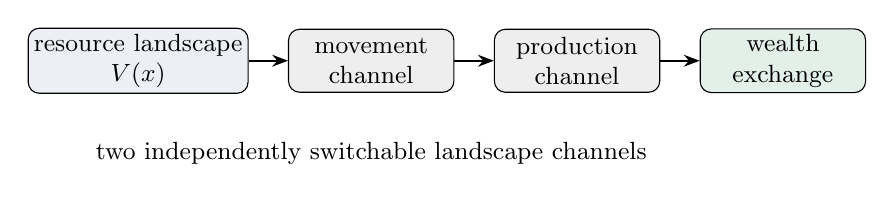
\begin{tikzpicture}[
  box/.style={draw, rounded corners, minimum width=21mm, minimum height=8mm, align=center, inner sep=2pt, font=\small},
  arrow/.style={-{Stealth[length=2.0mm]}, thick},
]
  \node[box, fill=accent!8] (terrain) {resource landscape\\ $V(x)$};
  \node[box, right=5mm of terrain, fill=grey!10] (move) {movement\\ channel};
  \node[box, right=5mm of move, fill=grey!10] (prod) {production\\ channel};
  \node[box, right=5mm of prod, fill=ok!12] (wealth) {wealth\\ exchange};
  \draw[arrow] (terrain) -- (move);
  \draw[arrow] (move) -- (prod);
  \draw[arrow] (prod) -- (wealth);
  \node[below=5mm of move, font=\small] {two independently switchable landscape channels};
\end{tikzpicture}
\caption{\textbf{Minimal causal chain.} The resource field can act through movement and production; wealth exchange is zero-sum and saturating.}
\label{fig:model}
\end{figure}

\begin{figure}[htbp]
\centering
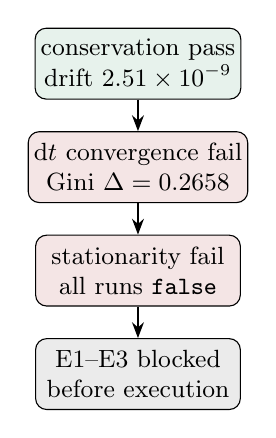
\begin{tikzpicture}[
  box/.style={draw, rounded corners, minimum width=26mm, minimum height=9mm, align=center, inner sep=2pt, font=\small},
  arrow/.style={-{Stealth[length=2.0mm]}, thick},
]
  \node[box, fill=ok!10] (conservation) {conservation pass\\ drift $2.51\times10^{-9}$};
  \node[box, below=4mm of conservation, fill=warn!12] (dt) {$\mathrm{d}t$ convergence fail\\ Gini $\Delta=0.2658$};
  \node[box, below=4mm of dt, fill=warn!12] (stat) {stationarity fail\\ all runs \texttt{false}};
  \node[box, below=4mm of stat, fill=grey!12] (stop) {E1--E3 blocked\\ before execution};
  \draw[arrow] (conservation) -- (dt);
  \draw[arrow] (dt) -- (stat);
  \draw[arrow] (stat) -- (stop);
\end{tikzpicture}
\caption{\textbf{Calibration-to-stop flow.} Passing conservation is necessary but not sufficient; the discretization and stationarity failures halt confirmatory runs.}
\label{fig:gate}
\end{figure}

\section{Discussion}

The conservation and non-negativity passes show that the exchange kernel's bookkeeping is correct. Total wealth is conserved to a maximum relative drift of $2.51\times10^{-9}$, no wealth becomes negative, and an equal-wealth state is absorbing under the symmetric rule. The two failures are distinct and actionable. The stationarity failure means the preregistered steady window (normalized drift $\le0.1$) is not reached within the allocated time; the $\mathrm{d}t$-convergence failure means the wealth distribution remains sensitive to halving the time step at $\mathrm{d}t=0.01$. Physically, the simulation has sound conservation but not yet a converged wealth distribution, so measuring a landscape effect would be premature.

We therefore make no claim that resource autocorrelation does or does not affect population structure. The correct scientific conclusion is narrower: the candidate parameter lock was non-final, E0 failed its calibration gate, and the confirmatory E1--E3 runs were never executed. This is an inconclusive cycle, not a null landscape result. The negative evidence itself has methodological value because the failure mode is visible only through a preregistered, outcome-blind gate. It points to a concrete repair path: revise the candidate lock using only runtime, numerical-stability, and outcome-blind health diagnostics; rerun E0 until conservation, non-negativity, $\mathrm{d}t$ convergence, and stationarity all pass; then resubmit E1--E3. Observed landscape effects from any blocked or future run must not be used to amend the current lock.

Limitations are explicit. Only $3$ pilot seeds and $25$ calibration runs were executed; the larger 80/160/120-run designs remain unused. The frozen SESOI is not authorized as a confirmatory threshold while convergence fails. The evidence boundary is a synthetic generative mechanism only: no claim about specific civilizations, states, empires, or historical causation is permitted. Reproduction, mortality, culture, technology, loyalty, conquest, taxation, and polity classification are disabled, so the results cannot speak to those mechanisms.

\section{Conclusion}

Cycle 1 produced an honest stop at the numerical-calibration layer. The minimal model conserves wealth and keeps it non-negative, but wealth observables fail preregistered stationarity and time-step convergence. Claim C1-NUM is contradicted as a joint claim; C2--C4 are inconclusive because no confirmatory runs were executed. The next step is an outcome-blind revision and recalibration before any landscape comparison. The full comprehensive record and all machine artifacts are preserved in the project repository, and no conclusion beyond the generative evidence boundary is asserted.

\begin{acknowledgments}
This PRL draft was generated by the isolated \texttt{journal\_prl} writing node from \texttt{research/orchestration/comprehensive.json}, \texttt{research/findings.json}, and \texttt{rules/journal-formats.md}. It introduces no new evidence and does not review its own draft.
\end{acknowledgments}

\begin{thebibliography}{4}
\bibitem{duran2025} M.~A. Dur\'an-Olivencia, \emph{The Emergence of Socio-Economic Structure: A First-Principles Kinetic Theory}, arXiv:2511.08742 (2025).
\bibitem{bae2026} S.~Bae et al., \emph{Unveiling hidden features of social evolution by inferring Langevin dynamics from data}, arXiv:2601.17772 (2026).
\bibitem{grimm2005} V.~Grimm et al., \emph{Pattern-oriented modeling of agent-based complex systems}, Science \textbf{310}, 987--991 (2005).
\bibitem{mcculloch2022} J.~McCulloch et al., \emph{Uncertainty quantification for agent-based models}, J. Artif. Soc. Soc. Simul. \textbf{25}(2), 1 (2022).
\end{thebibliography}

\end{document}
